\documentclass{SGGW-thesis}
\usepackage[utf8]{inputenc}
\usepackage{polski}
\selecthyphenation{polish}
\usepackage{amsmath}
\usepackage{amssymb}
\usepackage{hyperref}
\usepackage{url}
\usepackage{listings}
\usepackage{color}
\usepackage{textcomp}
\usepackage{tabularx}
\usepackage{graphicx}
\usepackage{hyperref}

\renewcommand{\lstlistingname}{Skrypt}
\lstdefinelanguage{JavaScript}{
  morekeywords=[1]{break, continue, delete, else, for, function, if, in, of, 
    new, return, this, typeof, var, void, while, with, let, const},
  % Literals, primitive types, and reference types.
  morekeywords=[2]{false, null, true, boolean, number, undefined,
    Array, Boolean, Date, Math, Number, String, Object, Set},
  % Built-ins.
  morekeywords=[3]{eval, parseInt, parseFloat, escape, unescape},
  sensitive,
  morecomment=[s]{/*}{*/},
  morecomment=[l]//,
  morecomment=[s]{/**}{*/}, % JavaDoc style comments
  morestring=[b]',
  morestring=[b]"
}[keywords, comments, strings]

% Requires package: color.
\definecolor{mediumgray}{rgb}{0.3, 0.4, 0.4}
\definecolor{mediumblue}{rgb}{0.0, 0.0, 0.8}
\definecolor{forestgreen}{rgb}{0.13, 0.55, 0.13}
\definecolor{darkviolet}{rgb}{0.58, 0.0, 0.83}
\definecolor{royalblue}{rgb}{0.25, 0.41, 0.88}
\definecolor{crimson}{rgb}{0.86, 0.8, 0.24}

\lstdefinestyle{JSES6Base}{
  backgroundcolor=\color{white},
  basicstyle=\ttfamily,
  breakatwhitespace=false,
  breaklines=false,
  captionpos=b,
  columns=fullflexible,
  commentstyle=\color{mediumgray}\upshape,
  emph={},
  emphstyle=\color{crimson},
  extendedchars=true,  % requires inputenc
  fontadjust=true,
  frame=single,
  identifierstyle=\color{black},
  keepspaces=true,
  keywordstyle=\color{mediumblue},
  keywordstyle={[2]\color{darkviolet}},
  keywordstyle={[3]\color{royalblue}},
  numbers=left,
  numbersep=5pt,
  numberstyle=\tiny\color{black},
  rulecolor=\color{black},
  showlines=true,
  showspaces=false,
  showstringspaces=false,
  showtabs=false,
  stringstyle=\color{forestgreen},
  tabsize=2,
  title=\lstname,
  upquote=true  % requires textcomp
}

\lstdefinestyle{JavaScript}{
  language=JavaScript,
  style=JSES6Base
}

\INZYNIERSKAtrue
\WZIMtrue

\title{Aplikacja webowa do udowadniania tautologii w~teorii
zbiorów}
\Etitle{Web application for proving tautologies in set theory}
\author{Aleksander Glebionek}
\date{2023}
\album{200810}
\thesis{Praca dyplomowa na kierunku:}
\course{Informatyka}
\promotor{dr. Andrzeja Zembrzuskiego}
\pworkplace{Instytut Informatyki Technicznej\\Katedra Systemów Informatycznych}


\begin{document}
\maketitle
\statementpage
\abstractpage
% polish
{Aplikacja webowa do udowadniania tautologii w~teorii
zbiorów}
{Celem pracy było stworzenie prostego i~intuicyjnego narzędzia do udowadniania tautologii w~teorii zbiorów. Zostało to zrealizowane w aplikacji webowej wykorzystującej czysty HTML, CSS i JavaScript. Opisane zostały podstawy teorii zbiorów, jej związek z logiką oraz metody dowodzenia tautologii. Omówiony został sposób działania aplikacji, odwrotna notacja polska, interesujące fragmenty kodu oraz wnioski dotyczące implementacji.}
{logika, teoria zbiorów, tautologia, odwrotna notacja polska, JavaScript}
% english
{Web application for proving tautologies in set theory}
{The goal of this paper was to create~a simple and intuitive tool for proving tautologies in set theory. This was accomplished in a web application using pure HTML, CSS and JavaScript. The basics of set theory, their relationship with logic, and methods for proving tautologies were described. The way the application works, reverse polish notation, interesting code fragments, and conclusions about the implementation were discussed.}
{logic, set theory, tautology, reverse polish notation, JavaScript}

\tableofcontents

\startchapterfromoddpage

\chapter{Wstęp}

\section{Cel, opis i motywacja stworzenia projektu\label{sec:1.1}}
\begin{paragraph}{}
    Celem aplikacji jest stworzenie prostego i~intuicyjnego narzędzia do udowadniania tautologii w~teorii zbiorów. Została stworzona przy użyciu czystych HTML, CSS i~JavaScript, czyniąc ją łatwą do uruchomienia i~zoptymalizowaną pod względem wydajności. Posiada ona graficzny interfejs w~stylu tradycyjnego kalkulatora, jednak zamiast używać cyfr i~operatorów arytmetycznych, używa liter oznaczających zbiory i~operatorów dla zbiorów. Posiada dodatkowo wybrane operacje logiczne oraz nawiasy.
    Aplikacja najpierw pobiera od użytkownika zdanie do sprawdzenia. Następnie generuje tabelkę wszystkich możliwych przypadków dla wszystkich zbiorów innych niż zbiór pusty. Dla każdego działania składającego się na podane zdanie wylicza jego wartość i~dodaje ją do tabelki. Finalnie wylicza wartości logiczne dla podanego działania. Jeżeli dla każdego przypadku wartość jest prawdą, to podane zdanie jest tautologią.
\end{paragraph}

\begin{paragraph}{}
    Podstawową motywacją do stworzenia tej aplikacji było dostarczenie przydatnego i~przystępnego narzędzia dla studentów uczących się logiki i~teorii zbiorów. Aplikacja jest przyjazna użytkownikowi i~intuicyjna, z~prostym interfejsem oraz możliwością używania klawiatury do wprowadzania zdań. Posiada również opcję wizualnego obejrzenia wygenerowanej przez program tabeli, oraz zawiera tabele prawdy dla operacji na zbiorach. Taka wizualizacja ma pomóc użytkownikom zrozumieć wynik programu, oraz pokazać połączenie między pozornie niepowiązanymi dziedzinami, jakimi są logika i~teoria zbiorów. Pobocznym celem było wykorzystanie przeze mnie okazji do testowania i~nauki różnych technik optymalizacyjnych. Finalnie, podczas moich pobieżnych poszukiwań, nie znalazłem nigdzie podobnej aplikacji. Dodatkowo mam nadzieję, że aplikacja znajdzie inne zastosowanie niż wyłącznie pomoc dla studentów.
\end{paragraph}
\newpage

\section{Tematyka i struktura pracy}

\begin{paragraph}{}
    Głównymi tematami pracy są logika i teoria zbiorów. W~ramach tej problematyki poruszane zostają dodatkowe kwestie niezbędne do realizacji i~zrozumienia aplikacji. W oparciu o~powyższe  zostało opisane jej działanie. Finalnie rozpatruje niektóre kawałki kodu oraz podsumowuje całość pracy.
\end{paragraph}

\begin{paragraph}{}
    Rozdział drugi skupia się na matematycznych podstawach działania aplikacji, to jest podstawach logiki, teorii zbiorów oraz powiązaniach obu tych dziedzin.
\end{paragraph}

\begin{paragraph}{}
    Rozdział trzeci zawiera opis działania aplikacji w oparciu o~przytoczoną w poprzednim rozdziale teorię oraz pozostałe tematy niezbędne do jej stworzenia, takie jak odwrotna notacja polska czy kolejność wykonywania działań.
\end{paragraph}

\begin{paragraph}{}
    Rozdział czwarty składa się z~istotnych lub ciekawych fragmentów kodu samej aplikacji oraz komentarza do nich.
\end{paragraph}

\begin{paragraph}{}
    Rozdział piąty to podsumowanie całej pracy, omówienie wydajności zastosowanego rozwiązania oraz rozważania co do alternatywnych metod wykazywania tautologii. 
\end{paragraph}


\chapter{Podstawy teoretyczne}

\section{Logika}

\begin{paragraph}{}
    Praca ma na celu utworzenie aplikacji do sprawdzania tautologii.  Niezbędna jest do tego znajmość podstawowych operacji logicznych, których tabele prawd przestawione są poniżej~\cite{ross2003discrete}.
\end{paragraph}

\begin{table}[h]
\vspace{1cm}

\parbox{.45\linewidth}{
    \centering

    $\begin{array}{|c|c|c|}
        \hline
        p & q & p \wedge q \\
        \hline
        0 & 0 & 0 \\
        0 & 1 & 0 \\
        1 & 0 & 0 \\
        1 & 1 & 1 \\
        \hline
    \end{array}$
    \caption{Koniunkcja}
}
\parbox{.45\linewidth}{
    \centering

    $\begin{array}{|c|c|c|}
        \hline
        p & q & p \vee q \\
        \hline
        0 & 0 & 0 \\
        0 & 1 & 1 \\
        1 & 0 & 1 \\
        1 & 1 & 1 \\
        \hline
    \end{array}$
    \caption{Alternatywa}
}

\vspace{1cm}

\parbox{.45\linewidth}{
    \centering

    $\begin{array}{|c|c|c|}
        \hline
        p & q & p \underline{\vee} q \\
        \hline
        0 & 0 & 0 \\
        0 & 1 & 1 \\
        1 & 0 & 1 \\
        1 & 1 & 0 \\
        \hline
    \end{array}$
    \caption{Alternatywa wykluczająca}
}
\parbox{.45\linewidth}{
    \centering

    $\begin{array}{|c|c|c|}
        \hline
        p & q & p \rightarrow q \\
        \hline
        0 & 0 & 1 \\
        0 & 1 & 1 \\
        1 & 0 & 0 \\
        1 & 1 & 1 \\
        \hline
    \end{array}$
    \caption{Implikacja}
}

\vspace{1cm}

\parbox{.45\linewidth}{
    \centering

    $\begin{array}{|c|c|c|}
        \hline
        p & q & p \leftrightarrow q \\
        \hline
        0 & 0 & 0 \\
        0 & 1 & 1 \\
        1 & 0 & 1 \\
        1 & 1 & 0 \\
        \hline
    \end{array}$
    \caption{Równoważność}
}
\parbox{.45\linewidth}{
    \centering

    $\begin{array}{|c|c|}
        \hline
        p & \sim p \\
        \hline
        0 & 1 \\
        1 & 0 \\
        \hline
    \end{array}$
    \caption{Negacja}
}
\end{table}

\begin{paragraph}{}
    Przykłady użycia zostaną podane w następnej sekcji, wraz z~definicjami działań na zbiorach jako przekształceń logicznych, korzystających z wyżej podanych spójników.
\end{paragraph}
\newpage


\newpage

\section{Teoria zbiorów\label{sec:2.2}}

\begin{paragraph}{}
    Zbiór jest pojęciem pierwotnym, co oznacza, że jest terminem, którego nie definiujemy. Możemy jednak określić konkretny zbiór poprzez określenie dziedziny i~warunku, który muszą spełniać jego elementy~\cite{wiki:Zbior}. Przykładowym zapisem może być: 
    \begin{equation}
        A = \{x \in \Omega: \Phi(x) \},
    \end{equation}
       w którym użyto następujących oznaczeń:\\
       $\Omega$ --- dziedzina, czyli zbiór zawierający wszystkie elementy na których operujemy, tzn. wszystkie możliwe wartości należące do zbioru $A$,~np. zbiór liczb naturalnych, \\
       $x$ --- element ze zbioru $\Omega$, \\
       $\Phi\left( x \right)$ --- warunek przynależności elementu $x$~do zbioru~$A$. 
\end{paragraph}

\begin{paragraph}{Przykład 2.2.1\label{ex:2.2.1}}
    Mając zbiory $A$ i $B$, zdefiniujmy zbiór $C$~w~następujący sposób:
    \begin{equation}
        C = \{x \in \Omega:\; x \in A \:\wedge\: x \in B\},
    \end{equation}
    gdzie $x \in A \:\wedge\: x \in B$ to warunek przynależności $\Phi\left( x \right)$. Należy zauważyć, że jest on funkcją zdaniową, tzn. dla każdej zmiennej zdaniowej $x \in A$ i $x \in B$ posiada wartość prawda albo fałsz. Stwórzmy dla niego tabelę prawdy.

    \begin{table}[h]
        \centering
        $\begin{array}{|c|c|c|}
            \hline
            x \in A & x \in B & x \in A \wedge x \in B \\
            \hline
            0 & 0 & 0 \\
            0 & 1 & 0 \\
            1 & 0 & 0 \\
            1 & 1 & 1 \\
            \hline
        \end{array}$
        \caption{Tabela prawdy dla $\Phi\left( x \right)$}
    \end{table}
\end{paragraph}

\begin{paragraph}{Przykład 2.2.2\label{ex:2.2.2}}
    Zademonstrujmy wykorzystanie powyższego warunku na praktycznym przykładzie, dla zbiorów operujących na liczbach naturalnych ($\Omega = \mathbb{N}$). Przykładowo, zdefiniujmy zbiory $A$ i $B$ w sposób następujący: $A = \{ 1, 2, 3 \},\; B = \{ 1 \}$. W takim przypadku, dla $x = 1$ stwierdzenia $x \in A $, $ x \in B$ i $ x \in A \wedge x \in B$ są prawdziwe. Zatem $x = 1$ należy do wynikowego zbioru $C$. Następnie, dla $x = 2$ zdanie $x \in A$ jest prawdziwe, a zdania $ x \in B$ i $ x \in A \wedge x \in B$ są fałszywe. Zatem $x = 2$ nie należy do zbioru $C$. Sytuacja wygląda identycznie dla $x = 3$. Finalnie więc $C = \{ 1 \}$, ponieważ tylko $x = 1$~spełnia warunek $\Phi(x)$.
\end{paragraph}

\begin{paragraph}{}
    Przykład~2.\ref{ex:2.2.2} zawiera kilka istotnych do zauważenia rzeczy. Po pierwsze, zbiór $C$~składa się z~elementów, które należą jednocześnie do zbiorów $A$~i~$B$.~Innymi słowy, jest to część wspólna tych zbiorów. Natomiast część wspólna zbiorów jest niczym innym, jak iloczynem. Zdefiniowaliśmy zatem warunek przynależności dla iloczynu zbiorów. Powinno więc być możliwe zdefiniowanie warunków przynależności dla pozostałych działań na zbiorach.
    Druga ważna obserwacja jest taka, że wynikiem iloczynu zbiorów również jest zbiór. Istnieją bowiem operacje, których wynikiem są wartości logiczne, na przykład operacje zawierania się zbiorów. Rozróżnienie to będzie istotne w dalszej części pracy.
    Trzecią obserwacją powinno być to, że wykorzystujemy trzeci wiersz z~tabelki prawdy dla naszego warunku przynaleźności zarówno dla $x=2$ jak i~$x=3$,~ponieważ wiersz ten dotyczy wszystkich takich $x$,~które należą do $A$~i~nie należą do $B$. Analogicznie dla wszystkich pozostałych wierszy w~tabeli. Finalnie warto zauważyć, że na podstawie tabelki prawdy dla warunku przynależności dla tego przykładu jesteśmy w stanie stwierdzić, że nie jest on tautologią.
    Wszystkie powyższe obserwacje i~rozróżnienia są niezwykle istotne zarówno dla teoretycznej, jak i~praktycznej części projektu. Poniżej znajdują się definicje warunków przynależności dla operacji na zbiorach wraz z~tabelami prawdy~\cite{ross2003discrete}. 
\end{paragraph}
 \begin{paragraph}{Uwaga:}
 W dalszej części, oznaczenie kolumny poprzez $A$~jest skrótem dla $x \in A$, natomiast zapis $A \cap B$ jest skrótem dla oznaczenia warunku przynależności $\Phi(x)$~dla iloczynu. Analogicznie dla pozostałych zbiorów i~operacji.
\end{paragraph}

\begin{paragraph}{}
    Operacje zwracające wartości logiczne:
\end{paragraph}

\begin{table}[h]
 \parbox{.45\linewidth}{
 \centering
 \begin{equation}
    A \subseteq B \iff x \in A \:\rightarrow\: x \in B
\end{equation}
        $\begin{array}{|c|c|c|}
            \hline
            A & B & A\subseteq B \\
            \hline
            0 & 0 & 1 \\
            0 & 1 & 1 \\
            1 & 0 & 0 \\
            1 & 1 & 1 \\
            \hline
            
        \end{array}$
    \caption{Podzbiór niewłaściwy}
}
\hspace{1.2cm}
 \parbox{.45\linewidth}{
 \centering
\begin{equation}
    A \subset B \iff x \in A \:\rightarrow\: x \in B\ \:\vee\: A \neq B
\end{equation}
        $\begin{array}{|c|c|c|}
            \hline
            A & B & A\subset B \\
            \hline
            0 & 0 & 0 \\
            0 & 1 & 1 \\
            1 & 0 & 0 \\
            1 & 1 & 0 \\
            \hline
        \end{array}$
    \caption{Podzbiór właściwy}
}
\end{table}

\newpage

 \begin{paragraph}{}
Operacje zwracające zbiory:
 \begin{table}[h]
 \parbox{.45\linewidth}{
 \centering
 \begin{equation}
    A \cup B = \{x \in \Omega:\; x \in A \:\vee\: x \in B\}
\end{equation}
        $\begin{array}{|c|c|c|}
            \hline
            A & B & A \cup B \\
            \hline
            0 & 0 & 0 \\
            0 & 1 & 0 \\
            1 & 0 & 0 \\
            1 & 1 & 1 \\
            \hline
            
        \end{array}$
    \caption{Suma zbiorów}
}
 \parbox{.45\linewidth}{
 \centering
\begin{equation}
    A \cap B = \{x \in \Omega:\; x \in A \:\wedge\: x \in B\}
\end{equation}


        $\begin{array}{|c|c|c|}
            \hline
            A & B & A \cap B \\
            \hline
            0 & 0 & 0 \\
            0 & 1 & 1 \\
            1 & 0 & 1 \\
            1 & 1 & 1 \\
            \hline
        \end{array}$
    \caption{Iloczyn zbiorów}
}
\parbox{.45\linewidth}{
 \centering
\begin{equation}
        A \setminus B = \{x \in \Omega:\; x \in A \:\wedge\: x \notin B\}
\end{equation}
        $\begin{array}{|c|c|c|}
            \hline
            A & B & A \setminus B \\
            \hline
            0 & 0 & 0 \\
            0 & 1 & 0 \\
            1 & 0 & 1 \\
            1 & 1 & 0 \\
            \hline
        \end{array}$
    \caption{Różnica zbiorów}
}
\hspace{1.2cm}
\parbox{.45\linewidth}{
\centering
\begin{equation}
    A' = \{x \in \Omega:\; \sim \left(x \in A \right)\}
\end{equation}
        \vspace{0.45cm}
        $\begin{array}{|c|c|c|}
            \hline
            A & A' \\
            \hline
            0 & 1 \\
            1 & 0 \\
            \hline
        \end{array}$
        \vspace{0.45cm}
    \caption{Dopełnienie zbiorów}
}
\end{table}
\end{paragraph}

\begin{paragraph}{}
    Należy zauważyć, że w~powyższych operacjach rozważane są wszystkie możliwe wartości dla zmiennych zdaniowych stwierdzających, że $x$ należy do jakiegoś zbioru. Zdanie $x \in \emptyset$ nie byłoby w tym przypadku zmienną, a~stałą, ponieważ zawsze posiada wartość logiczną fałsz. Dodatkowo warto zwrócić uwagę, że obecność zbioru pustego w~rozpatrywanym zdaniu nie oznacza, że pozostałe zbiory nie mogą być puste.
\end{paragraph}

\newpage

\section{Tautologie i ich naiwne udowadnianie}

\begin{paragraph}{}
    Ostatnią obserwacją dla Przykładu~\ref{ex:2.2.2}.2 był fakt, że omawiany tam warunek przynależności nie jest tautologią. Tautologią nazywamy takie wyrażenie, które jest zawsze prawdziwe, niezależnie od wartości logicznych zmiennych zdaniowych z~których się składa~\cite[rozdz.~2.2]{ross2003discrete}.
\end{paragraph}

\begin{paragraph}{Przykład 2.3.1\label{ex:2.3.1}}
    Rozważmy następującą tautologię.

\begin{equation}
            \underbrace{A \cap B \: = \: A \setminus C}_L 
        \;\rightarrow\;
            \underbrace{A \cap B \cap C \: = \: \emptyset}_R
        \label{eq:example_tautology}
    \end{equation}
\begin{table}[h]
 \centering
        $\begin{array}{|c|c|c|c|c|c|c|c|c|c|}
            \hline
            A & B & C & \emptyset & A \cap B & A \setminus C & L & A \cap B \cap C & R & L \rightarrow R \\
            \hline
            0 & 0 & 0 & 0 & 0 & 0 & 1 & 0 & 1 & 1 \\
            0 & 0 & 1 & 0 & 0 & 0 & 1 & 0 & 1 & 1 \\
            0 & 1 & 0 & 0 & 0 & 0 & 1 & 0 & 1 & 1 \\
            0 & 1 & 1 & 0 & 0 & 0 & 1 & 0 & 1 & 1 \\
            1 & 0 & 0 & 0 & 0 & 1 & 0 & 0 & 1 & 1 \\
            1 & 0 & 1 & 0 & 0 & 0 & 1 & 0 & 1 & 1 \\
            1 & 1 & 0 & 0 & 1 & 1 & 1 & 0 & 1 & 1 \\
            1 & 1 & 1 & 0 & 1 & 0 & 0 & 1 & 0 & 1 \\
            \hline
        \end{array}$
        \caption{Tabela prawdy dla równania (2.9)}
        \label{table:example_tautology}
\end{table}
\end{paragraph}
\begin{paragraph}{}
    Powyższa tabela dowodzi, że równanie~\eqref{eq:example_tautology} jest w~istocie tautologią, ponieważ w ostatniej kolumnie znajdują się same jedynki.
    Aby wykonać powyższy dowód, należy najpierw określić unikalne zbiory wchodzące w~jego skład, inne niż zbiór pusty.
    W~kolejnym kroku dla każdego z~tych zbiorów wypisujemy wierszami wszystkie możliwe wartości logiczne dla zdania, czy $x$~należy do danego zbioru. Następnie dla każdego działania składającego się na początkowe zdanie wyznaczamy jego wartość logiczną dla każdego możliwego przypadku. 
    Sprawdzenie kończy się na sprawdzeniu wartości logicznych dla początkowego zdania. Jest ono tautologią wtedy i~tylko wtedy, gdy jest prawdziwe dla wszystkich możliwych przypadków.

    Dla $n$~zbiorów mamy do rozważenia $2^{n}$~możliwych przypadków. Z~tego powodu powyższy dowód tabelkowy został określony jako naiwny, ponieważ dla zdania składającego się z~dziesięciu zbiorów trzeba sprawdzić $2^{10}=1024$~przypadki, pomnożone przez liczbę operacji składających się na zdanie.

    W następnym rozdziale powyższy proces zostanie omówiony dokładniej, aby móc go zrealizować w~aplikacji.
\end{paragraph}

\chapter{Przenoszenie teorii na praktykę}

\section{Przechowywanie i operowanie na tabeli\label{sec:3.1}}

\begin{paragraph}{}
    Ponieważ dowód wykorzystywany w~aplikacji będzie opierał się na metodzie tabelkowej, podstawowym pytaniem jest, w~jaki sposób przechowywać tabelę, aby móc łatwo na niej operować.

    Wykorzystane w~aplikacji rozwiązanie to słownik tablic. Kluczami słownika są nazwy kolumn np. $A$,~$B$,~$\emptyset$,~natomiast wartościami są tablice 32 bitowych liczb całkowitych.

    Aby operować na tabeli w~takiej formie, należy iterować po liczbach w jednej tablicy i~wykonywać bitowe operacje między liczbami na tych samych indeksach w drugiej tablicy. Długość pojedynczej tablicy to $\lceil 2^{n} / 32 \rceil$, gdzie $n$ to liczba zbiorów innych niż zbiór pusty w~sprawdzanym zdaniu.

    Ponieważ tabela operuje na zerach i~jedynkach, opisany powyżej sposób jest najbardziej optymalną metodą jej przechowywania, zarówno ze względów pamięciowych jak i~operacyjnych, tzn. komputer może bez problemu wykonać operacje pomiędzy bitami dwóch liczb.
\end{paragraph}

\section{Generowanie wszystkich możliwych przypadków}

\begin{paragraph}{}
    Skoro wiadomo, jak ma wyglądać struktura do przechowywania tabeli, należy zastanowić się, w~jaki sposób poprawnie ją wygenerować.

    Rozpocząć należy od zidentyfikowania wszystkich unikalnych zbiorów w~zdaniu innych niż zbiór pusty. Ponieważ w~kodzie zdanie będzie zapisane jako łańcuch znaków, należy policzyć, ile unikalnych wielkich liter alfabetu łacińskiego się w~nim znajduje. Następnie należy wygenerować liczby, których bity odpowiadają zerom i~jedynkom w kolumnach tabeli. W~jaki sposób tego dokonać?

    Aby odpowiedzieć na to pytanie, można spojrzeć do przykładu~\ref{ex:2.3.1}.1. Dla równania \eqref{eq:example_tautology} można znaleźć trzy litery --- $A$,~$B$~i~$C$. Po przypatrzeniu się tabeli~\ref{table:example_tautology}, można zauważyć prostą zależność między jej wierszami. Ponumerujmy je od góry do dołu zaczynając od zera. Niech $i$~oznacza numer wiersza. Wartości kolumn w~wierszu $i$~odpowiadają bitom w~zapisie binarnym liczby $i$,~w~taki sposób, że $i_{(10)} = ABC_{(2)}$. Przykładowo, dla wiersza o~$i = 3$, kolumna $A$~ma wartość $0$, a~kolumny $B$~i~$C$~wartość $1$. Jak widać, $3_{(10)} = 011_{(2)}$.

    Powyższy fakt można wykorzystać do wygenerowania tabeli. Liczby zapisane są w~pamięci komputera w~postaci binarnej. Wykonując w~kodzie pętlę od $i = 0$ do $i = 2^{n}-1$, gdzie $n$ to liczba zbiorów innych niż zbiór pusty, można odczytać bity każdej z~tych liczb i~umieścić je w~odpowiednich kolumnach. Pojawia się pytanie, w~jaki sposób odczytać bit na konkretnym miejscu.

    Niech $m$~oznacza indeks bitu zapisanej dwójkowo liczby. Dodatkowo, niech rozpoczyna się on od zera i~od prawej strony liczby, w~taki sposób, że dla kolumny $C$ $m=0$, dla $B$ $m=1$, a~dla $A$~$m=2$. Aby odczytać bit liczby $i$ na pozycji $m$, należy najpierw przesunąć jej bity o $m$~miejsc w~prawo, a~następnie dokonać koniunkcji między bitami wyniku a~jedynką, aby wyzerować wszystkie bity oprócz najmniej znaczącego.
\end{paragraph}

\begin{paragraph}{Przykład 3.2.1\label{ex:3.2.3}}
    We wcześniejszym przykładzie wartości kolumn $A$, $B$ i $C$ dla wiersza o~$i = 3$ odczytano z tabeli. Komputer wie, że $3_{(10)} = 011_{(2)}$. Spróbujmy wykorzystać ten fakt, aby automatycznie generować kolumny. Dla $m=0$, przesunięcie liczby $011_{(2)}$ o~zero miejsc w~prawo nie zmienia jej. Bitowa koniunkcja z~jedynką zwraca $001_{(2)}$. $001_{(2)} = 1_{(10)}$. Zatem dla rozpatrywanego wiersza kolumna $C$ ma wartość $1$. Dla $m=1$, przesunięcie liczby $011_{(2)}$ o~jedno miejsce w~prawo daje $001_{(2)}$. Bitowa koniunkcja z~jedynką zwraca $001_{(2)}$. $001_{(2)} = 1_{(10)}$. Zatem dla rozpatrywanego wiersza kolumna $B$~ma wartość $1$. Dla $m=2$, przesunięcie liczby $011_{(2)}$ o~dwa miejsca w~prawo daje $000_{(2)}$. Bitowa koniunkcja z~jedynką zwraca $000_{(2)}$. $000_{(2)} = 0_{(10)}$. Zatem dla rozpatrywanego wiersza kolumna $A$~ma wartość $0$.
\end{paragraph}

\begin{paragraph}{}
    Powyższy przykład ilustruje, jak przy użyciu prostej pętli i manipulacji bitowych można wygenerować wiersze tabeli. W podrozdziale \ref{sec:3.1} powiedziane jednak zostało, że w kodzie tabela jest przechowywana kolumnami, gdzie jedna kolumna to tablica 32-bitowych liczb całkowitych. Dodatkowo, tablice te to wartości słownika, którego kluczami są nazwy zbiorów, których dotyczą. Przyjęte zostało, że najbardziej znaczący bit w~32-bitowej liczbie odpowiada pierwszemu wierszowi w~kolumnie. Otrzymany bit na danej pozycji będzie najmniej znaczącym z~32~bitów. Na pozostałych bitach będą zera. Aby umieścić go na odpowiedniej pozycji, należy przesunąć go w~lewo o~$32 - 1 - i$. Przesunięcia należy dokonać na otrzymanym wyniku. Aby włączyć go do obecnej wartości kolumny, należy dokonać między nimi bitowej alternatywy.
    
    Mając na uwadze wszystkie powyższe informacje, algorytm generowania wszystkich możliwych przypadków można przedstawić poniższymi krokami.
    \begin{enumerate}
        \item Znajdujemy w rozpatrywanym zdaniu wszystkie wielkie litery alfabetu łacińskiego. Oznaczmy ich liczbę przez $n$. Zapisujemy je w \emph{tablicy liter} i sortujemy ją alfabetycznie.
        \item Tworzymy wstępny \emph{słownik}, którego kluczami są znalezione litery, a wartościami tablice o długości $\lceil 2^{n} / 32 \rceil$ wypełnione zerami. Ustawiamy \emph{indeks} dla tych tablic na zero.
        \item Odwracamy kolejnością \emph{tablicę liter}.
        \item Ustawiamy początkowe \emph{przesunięcie} na 31.
        \item Wykonujemy pętlę od $i=1$ do $i=2^{n}-1$. Dla każdej iteracji:
        \begin{enumerate}
            \item Zapisujemy obecną wartość $i$ do \emph{zmiennej pomocniczej};
            \item Wykonujemy pętlę po literach \emph{tablicy liter}. Dla każdej \emph{litery}:
            \begin{enumerate}
                \item Obliczamy wartość najmniej znaczącego bitu dla \emph{zmiennej pomocniczej} poprzez bitową koniunkcję z jedynką;
                \item Przesuwamy bitowo otrzymaną liczbę w lewo o \emph{przesunięcie};
                \item Wykonujemy bitową alternatywę między wartością \emph{słownika} dla obecnej \emph{litery} na odpowiednim \emph{indeksie} a przesuniętą wcześniej wartością;
                \item Przesuwamy \emph{tymczasową zmienną} o jeden bit w prawo, aby bit na kolejnej pozycji stanowił teraz najmniej znaczący.
            \end{enumerate}
            \item Zmniejszamy wartość \emph{przesunięcia} o jeden;
            \item Jeżeli wykorzystaliśmy wszystkie 32 bity w obecnej liczbie w tablicy (czyli jeżeli reszta z dzielenia $i + 1$ przez $32$ wynosi $0$) to zwiększamy $indeks$ o $1$ i ustawiamy \emph{przesunięcie} ponownie na wartość $31$.
        \end{enumerate}
        \item Na koniec sprawdzamy, czy w rozpatrywanym zdaniu znajduje się zbiór pusty. Jeżeli tak, do dodajemy go do \emph{słownika} jako klucz, a jego wartość ustawiamy na tablicę wypełnioną zerami.
    \end{enumerate}
\end{paragraph}

\section{Odwrotna Notacja Polska}

\begin{paragraph}{}
    Operacje bitowe komputer jest w stanie wykonywać bardzo szybko. Pojawia się jednak problem z wytłumaczeniem komputerowi, w jaki sposób poprawnie wykonywać owe operacje zgodnie z intencjami użytkownika --- w dobrej kolejności, uwzględniając nawiasy, między poprawnymi zbiorami, etc.

    Stworzenie kodu, który rozwiązuje równania w notacji używanej na co dzień, w której operator znajduje się pomiędzy argumentami, tzw. notacji infiksowej, jest skomplikowanym problemem. Na szczęście nie trzeba tego robić. Można bowiem przekonwertować zapis z~notacji infiksowej do notacji posfiksowej, w której operator jest za argumentami. Notacja ta, znana jako Odwrotna Notacja Polska (RPN), pozwala komputerowi łatwo wykonywać działania. Wynika to z faktu, że notacja postfiksowa zawiera w sobie informacje co do kolejności wykonywania działań~\cite{wiki:Reverse_Polish_notation}.

    Zanim przedstawiony zostanie algorytm rozwiązywania takich równań, należy wprowadzić pojęcie tokenu. W ramach pracy, tokenem będzie określany fragment działania, który posiada identyfikowalny rodzaj i wartość~\cite{wiki:Token}. Przykładowo, w działaniu $34+1$, tokenami od lewej do prawej będzie $34$, będący tokenem liczby o takiej wartości, $+$ będący tokenem operatora dodawania oraz $1$, ponownie będący tokenem liczby. Tokeny mogą mieć różną długość i powinny być łatwo identyfikowalne, tzn. wiadomym jest, że we wcześniejszym przykładzie liczba $34$ stanowi pojedynczy token, a nie są to dwa oddzielne tokeny $3$ i $4$. W~aplikacji tokeny zawsze mają długość jeden, co ułatwia jej działanie.
    
    Algorytm rozwiązywania równań w postaci postfiksowej można przedstawić w następujących krokach:
    \begin{enumerate}
    \item Odczytujemy tokeny po kolei od lewej do prawej strony.
    \item Gdy natrafimy na token operatora:
        \begin{enumerate}
            \item Sprawdzamy iluargumentowy jest operator;
            \item Bierzemy odpowiednią liczbę argumentów na lewo od operatora i wykonujemy między nimi znalezioną operację;
            \item Tokeny użyte do wykonania operacji zastępujemy wynikiem.
        \end{enumerate}
    \item Powtarzamy czynność aż pozostanie jeden token, będący wynikiem równania.
    \end{enumerate}
\end{paragraph}

\begin{paragraph}{Przykład 3.3.1\label{ex:3.3.1}} Rozpatrzmy działanie $3 + (4 * 2):$
    
    Działanie w Odwrotnej Notacji Polskiej ma postać $3$ $4$ $2$ $*$ $+$.
    \begin{enumerate}
        \item Czytamy tokeny od lewej strony.
        \item Pierwszym znalezionym operatorem jest mnożenie.
        \begin{enumerate}
            \item Operator mnożenia jest dwuargumentowy;
            \item Bierzemy zatem dwa operatory na lewo od niego, czyli $4$ i $2$ i mnożymy je, otrzymując $8$;
            \item Zastępujemy użyte tokeny otrzymanym wynikiem. Działanie ma teraz postać $3$ $8$ $+$.
        \end{enumerate}
        \item Czytamy tokeny od miejsca w którym skończyliśmy, czyli od liczby $8$.
        \item Natrafiamy na operator dodawania.
        \begin{enumerate}
            \item Operator dodawania jest dwuargumentowy;
            \item Bierzemy zatem dwa operatory na lewo od niego, czyli $3$ i $8$ i dodajemy je, otrzymując $11$;
            \item Zastępujemy użyte tokeny otrzymanym wynikiem. Działanie ma teraz postać $11$.
        \end{enumerate}
        \item $11$ jest ostatnim tokenem i tym samym wynikiem działania. 
    \end{enumerate}

    Powyższy przykład odnosi się do liczb. W aplikacji pojedyncze liczby zastąpione są tablicami bitów, a operacje na liczbach operacjami bitowymi.

    Aby zrealizować algorytm, należy najpierw zdefiniować dodatkowe struktury. \emph{Słownik} będzie zawierać wygenerowane przypadki dla zbiorów, a \emph{stos} to struktura pomocnicza do przechowywania używanych do obliczeń tablic. Całość aglorytmu można przedstawić następująco:
    \begin{enumerate}
        \item Czytamy tokeny od lewej strony.
        \item Jeżeli token jest zbiorem:
        \begin{enumerate}
            \item Wyszukujemy jego wartość w \emph{słowniku};
            \item Dodajemy znalezioną wartość do \emph{stosu}.
        \end{enumerate}
        \item Jeżeli token jest operatorem dopełnienia:
        \begin{enumerate}
            \item Zdejmujemy tablicę ze \emph{stosu};
            \item Iterujemy po jej zawartości i negujemy wszytkie jej bity;
            \item Dodajemy zanegowaną tablicę na \emph{stos}.
        \end{enumerate}
        \item Jeżeli token jest operatorem innym niż operator dopełnienia, tj. operatorem dwuargumentowym:
        \begin{enumerate}
            \item Zdejmujemy ze \emph{stosu} pierwszą tablicę jako prawy argument operacji;
            \item Zdejmujemy ze \emph{stosu} drugą tablicę jako lewy argument operacji;
            \item Wykonujemy znalezioną operację między bitami liczb na tych samych indeksach w zdjętych tablicach;
            \item Dodajemy wynik na \emph{stos}.
        \end{enumerate}
        \item Wykonujemy algorytm tak długo aż skończą się tokeny.
    \end{enumerate}
\end{paragraph}

\begin{paragraph}{Uwaga:}
    W punkcie $4.$ strona argumentu ma znaczenie przez kolejność niektórych operacji na zbiorach, np. $A \setminus B$ to nie to samo co $B \setminus A$.
\end{paragraph}

\begin{paragraph}{Przykład 3.3.2\label{ex:3.3.2}}
Rozpatrzmy działanie $A \cap B = \emptyset$. W Odwrotnej Notacji Polskiej ma ono postać $A$ $B$ $\cap$ $\emptyset$ $=$. Przypomnijmy tabelkę możliwych przypadków dla tych zbiorów.
    
    \begin{table}[h]
        \centering
        $\begin{array}{|c|c|}
            \hline
            A & B \\
            \hline
            0 & 0 \\
            0 & 1 \\
            1 & 0 \\
            1 & 1 \\
            \hline
        \end{array}$
        \caption{Tabela możliwych przypadków dla zdania zawierającego tylko zbiory $A$ i $B$}
    \end{table}  
    
    Dla uproszczenia przyjmijmy, że jedna liczba w tablicy jest dwubitowa, aby łatwiej zilustrować zasadę działania. Dodatkowo załóżmy, że górą stosu jest jego prawa strona. W takim razie wygenerowany \emph{słownik} ma następującą postać:
    $\{ A: \left[ 00, 11 \right], B: \left[ 01, 01 \right], \emptyset: \left[00, 00 \right]\}$. Algortym dla tego przypadku będzie przebiegał następujaco:
    \begin{enumerate}
        \item Czytamy tokeny od lewej strony.
        \item Pierwszym tokenem jest $A$:
        \begin{enumerate}
            \item Odczytujemy w \emph{słowniku} wartość dla klucza $A$, która wynosi [00, 11];
            \item Dodajemy ją na \emph{stos}, który teraz ma postać [[00, 11]].
        \end{enumerate}
        \item Kolejnym tokenem jest $B$:
        \begin{enumerate}
            \item Odczytujemy w \emph{słowniku} wartość dla klucza $B$, która wynosi [01, 01];
            \item Dodajemy ją na \emph{stos}, który teraz ma postać [[00, 11], [01, 01]].
        \end{enumerate}
        \item Kolejnym tokenem jest $\cap$:
        \begin{enumerate}
            \item Zdejmujemy ze \emph{stosu} pierwszą tablicę, która ma wartość [01, 01] i traktujemy ją jako prawy argument operacji;
            \item Zdejmujemy ze \emph{stosu} drugą tablicę, która ma wartość [00, 11] i traktujemy ją jako lewy argument operacji;
            \item Wykonujemy między bitami w tablicach operację logiczną będącą warunkiem przynależności dla sumy zbiorów, otrzymując w wyniku tablicę [00, 01];
            \item Dodajemy wynik na \emph{stos}, który teraz ma postać [[00, 01]].
        \end{enumerate}
        \item Kolejnym tokenem jest $\emptyset$.
        \begin{enumerate}
            \item Odczytujemy w \emph{słowniku} wartość dla klucza $\emptyset$, która wynosi [00, 00];
            \item Dodajemy ją na \emph{stos}, który teraz ma postać [[00, 01], [00, 00]].
        \end{enumerate}
        \item Kolejnym tokenem jest $=$.
        \begin{enumerate}
            \item Zdejmujemy ze \emph{stosu} pierwszą tablicę, która ma wartość [00, 01] i traktujemy ją jako prawy argument operacji;
            \item Zdejmujemy ze \emph{stosu} drugą tablicę, która ma wartość [00, 00] i traktujemy ją jako lewy argument operacji;
            \item Wykonujemy między bitami w tablicach operację logiczną będącą operacją równoważności dla bitów, otrzymując w wyniku tablicę [11, 10];
            \item Dodajemy wynik na \emph{stos}, który teraz ma postać [[11, 10]].
        \end{enumerate}
        \item Token $=$ był ostatnim tokenem. Na stosie została jedna tablica, będąca wynikiem działania. Jeżeli wszystkie bity w tej tablicy są jedynkami, oznacza to, że rozpatrywane działanie jest tautologią. Dla tego przykładu widzimy, że nie jest to tautologia.
    \end{enumerate}
    Jak widać na powyższym przykładzie, algorytm jest prosty, zatem będzie prosty do zakodowania. Pojawia się pytanie, w jaki sposób dokonać konwersji do notacji postfiskowej?
\end{paragraph}

\section{Kolejność wykonywania działań}

\begin{paragraph}{}
    Aby poprawnie przekształcać równania do Odwrotnej Notacji Polskiej, niezbędna jest znajomość kolejności wykonywania działań. Jak wygląda ona dla zbiorów i czy w ogóle jest istotna?

    Należy tutaj cofnąć się do rozdziału drugiego. Drugim wnioskiem z przykładu \ref{ex:2.2.2}.2 jest różnica w tym co zwracają operacje na zbiorach. Aby lepiej to zrozumieć, można spojrzeć na równanie w przykładzie \ref{ex:2.3.1}.1. Jego sens można wyrazić słownie w sposób następujący: \emph{Jeżeli zbiór $A \cap B$ jest równy zbiorowi $A \setminus C$, to czy z tego wynika, że zbiór $A \cap B \cap C$ jest zbiorem pustym?}

    Aby poprawnie odpowiedzieć na to pytanie, najpierw trzeba wyliczyć zbiory, potem je porównać, a na koniec sprawdzić implikację. Wynika z tego zatem, że priorytety działań wyglądają w sposób następujący, od największego do najmniejszego:
    \begin{enumerate}
        \item Suma, różnica, iloczyn,
        \item Równość, operacje zawierania, podzbiory,
        \item Implikacja, równoważność.
    \end{enumerate}

    Nie wyczerpuje to jednak wszystkich działań. Istnieje jeszcze jednoargumentowy operator dopełnienia zbioru. Zakłada się, że zapis $A \cup B'$ oznacza sumę zbiorów $A$ i dopełnienia zbioru $B$. Operator dopełnienia też zwraca zbiór, ma jednak wyższy priorytet od operacji dwuargumentowych. Aby zapisać dopełnienie sumy zbiorów, wówczas sumę należy ująć w~nawiasy, otrzymując $\left( A \cup B \right)'$. Nawiasy zawsze mają najwyższy priorytet.

    Finalnie zatem kolejność wykonywania działań dla aplikacji prezentuje się następująco:
    \begin{enumerate}
        \item Nawiasy,
        \item Dopełnienie zbioru,
        \item Suma, różnica, iloczyn,
        \item Równość, operacje zawierania, podzbiory,
        \item Implikacja, równoważność.
    \end{enumerate}
\end{paragraph}

\section{Konwersja do Odwrotnej Notacji Polskiej}

\begin{paragraph}{}
    Mając zdefiniowaną kolejność działań, można wreszcie przejść do omówienia w jaki sposób konwertować działania z notacji infiksowej do postfiksowej.

    Powszechnym rozwiązaniem jest aglorytm Shunting-Yard. Pseudokod algorytmu można znaleźć w sekcji ,,The algorithm in detail'' na stronie~\cite{wiki:Shunting_yard_algorithm}. Ponieważ jednak odnosi się on w~ogólności do liczb, a nie do ograniczonej liczby możliwych operacji na zbiorach, należy go zmodyfikować, aby odpowiadał potrzebom aplikacji.
\end{paragraph}

\begin{paragraph}{Algorytm Shunting-Yard dla zbiorów\\}
    \emph{Wynik} to łańcuch znaków zawierający przekonwertowane działanie, a \emph{stos} to struktura pomocnicza do przechowywania tokenów.

    \begin{enumerate}
        \item Czytamy tokeny od lewej strony.
        \item Jeżeli token jest zbiorem, dodajemy go do \emph{wyniku}.
        \item Jeżeli token jest lewym nawiasem, dodajemy go do \emph{stosu}.
        \item Jeżeli token jest prawym nawiasem, to zdejmujemy ze \emph{stosu} tokeny i dodajemy do \emph{wyniku} tak długo, aż nie natrafimy na lewy nawias. Lewy nawias zdejmujemy ze \emph{stosu}, ale nie dodajemy go do wyniku.
        \item Jeżeli token jest operatorem i jeżeli \emph{stos} nie jest pusty, zdejmujemy z niego tokeny i~dodajemy je do \emph{wyniku} tak długo, aż nie natrafimy na lewy nawias lub nie opróżnimy \emph{stosu}. Na koniec dodajemy token do \emph{stosu}.
    \end{enumerate}

    W powyższym algorytmie w żadnym miejscu nie pojawia się kwestia kolejności wykonywania działań. Wynika to z~faktu, że powyższa wersja algorytmu odpowiada tej w~programie~i zakłada, że konwertowane zdanie jest wcześniej odpowiednio zmodyfikowane.

    Modyfikacja polega na dodawaniu do zdania nawiasów w~taki sposób, aby kolejność działań wynikała bezpośrednio z~nich~\cite{wiki:Operator-precedence_parser}.
\end{paragraph}

\begin{paragraph}{Algorytm dodawania nawiasów\\}
    \emph{Wynik} jest łańcuchem znaków, na początek którego dodajemy pięć lewych nawiasów. 
    \begin{enumerate}
        \item Czytamy tokeny od lewej strony.
        \item Jeżeli token jest nawiasem, dodajemy do \emph{wyniku} cztery takie same nawiasy.
        \item Jeżeli token jest operacją sumy, różnicy albo ilocznu, dodajemy go do \emph{wyniku} w formie `)token(`.
        \item Jeżeli token jest operacją równości albo zawierania, dodajemy go do \emph{wyniku} w formie `))token((`.
        \item Jeżeli token jest operacją implikacji albo równoważności, dodajemy go do \emph{wyniku} w~formie `)))token(((`.
        \item Jeżeli token jest zbiorem albo operacją dopełnienia, dodajemy go bezpośrednio do wyniku, bez dodatkowych nawiasów. Fakt, że robimy to dla dopełenienia wynika z~faktu, że jest to operator jednoelementowy, który zawsze znajduje się bezpośrednio przy elemencie którego ma dotytyczyć.
    \end{enumerate}

    Na koniec dodajemy do \emph{wyniku} pięć prawych nawiasów, aby zrównoważyć te dodane na początku.
    
    Stosując powyższy algorytm do równania 2.9, otrzymujemy wynik w postaci:
    \begin{equation}
            \left( \left( \left( \left(
            \left( A \right) 
            \cap 
            \left( B \right)
            \right) \: = \: \left(
            \left( A \right) 
            \setminus 
            \left( C \right)
            \right) \right) \;\rightarrow\; \left( \left( 
            \left( A \right) 
            \cap 
            \left( B \right)
            \cap
            \left( C \right)
            \right) \: = \: \left(
            \left( \emptyset \right) \right) \right) \right) \right).
        \label{eq:example_tautology_parenthesized}
    \end{equation}

    Bez wykonywania powyższej modyfikacji, należałoby uwzględnić w algorytmie konwersji sprawdzanie pierwszeństwa operatorów oraz pojawiłaby się dodatkowa kwestia asocjatywności operatorów, która dla uproszczenia zostaje pominięta.
\end{paragraph}



\chapter{Implementacja algorytmów w kodzie\label{sec:4}}

\section{Kilka słów o JavaScript}

\begin{paragraph}{}
    Aplikacja ma działać w przeglądarce bez potrzeby instalowania dodatkowego oprogramowania. Z tego powodu, kod niezbędny do jej działania napisany jest w języku JavaScript.

    Język ten posiada wbudowane i łatwe w obsłudzie struktury oraz operatory niezbędne do realizacji opisanych w poprzednim rozdziale algorytmów, takie jak słowniki czy operatory bitowe. Poniżej znajduje się lista użytych operatorów:
    \begin{itemize}
        \item $a \& b$ --- koniunkcja między bitami liczb $a$ i $b$
        \item $a | b$ --- alternatywa między bitami liczb $a$ i $b$
        \item $a \string^ b$ --- alternatywa wykluczająca między bitami liczb $a$ i $b$
        \item $a << n$ --- przesunięcie bitow liczby $a$ o $n$ miejsc w lewo
        \item $a >> n$ --- przesunięcie bitow liczby $a$ o $n$ miejsc w prawo
        \item $\sim a$ --- negacja bitów liczby $a$
    \end{itemize}
    
    Aplikacja będzie musiała wyświetlać symbole logiki i teorii zbiorów. Ponieważ symbole te nie są wykorzystywane na co dzień, w kodzie zdefiniowany został słownik o nazwie \emph{symbols}, którego kluczem jest nazwa symbolu, np. ,,emptySet'', a wartością kod Unicode tego symbolu. Unicode to międzynarodowy standard kodowania znaków, który przypisuje unikalny identyfikator numeryczny do większości używanych na świecie liter czy symboli matematycznych~\cite{wiki:Unicode}. Umożliwia on jednoznaczne reprezentowanie i przetwarzanie różnych języków, pism i symboli na komputerze, niezależnie od używanej platformy i języka systemu. 
    Różne czcionki obsługują różne symbole Unicode, ponieważ każda czcionka zawiera tylko określony zestaw znaków. Nie wszystkie czcionki zawierają wszystkie znaki Unicode, więc konieczne jest wybieranie czcionek, które posiadają potrzebne symbole. Na potrzeby tej aplikacji została w niej zawarta czcionka Arial, która posiada wszystkie niezbędne symbole.
    Dodatkowo, na przestrzeni pracy mówione jest, że liczby kolumny to tablice 32-bitowych liczb całkowitych. Zaglądając do dokumentacji Mozilli można zauważyć informację, że JavaScript przechowuje wszystkie liczby jako 64-bitowe, zmiennoprzecinkowe liczby podwójnej precyzji. Niżej jednak, w tej samej dokumentacji, można przeczytać, że operatory bitowe zawsze konwertują argumenty do 32-bitowych liczb całkowitych~\cite{docs:mozilla:numbers}.
\end{paragraph}
\newpage
\section{Algorytm generacji przypadków}

\begin{lstlisting}[style=JavaScript, caption={Kod generujący słownik tablic wszystkich możliwych przyadków}]
//look for letters to determine how many unique sets we have
const sets = [...new Set(sentence.match(/[A-Z]/g))].sort();

//initialize binaries object and calculate necessary data
const binaries = {};
const numberOfCases = 2 << sets.length - 1; //2^sets.length
const arraySize = Math.ceil(numberOfCases / 32);
for (const set of sets) binaries[set] = [];

//generate binaries for all possible cases
sets.reverse()
let auxilary;
let index = 0;
let shift = 31;
for (let i = 0; i < numberOfCases; i++) {
    auxilary = i;
    for (const set of sets) {
        binaries[set][index] |= (auxilary & 1) << shift;
        auxilary >>= 1;
    }
    shift--;
    if ((i + 1) % 32 === 0) {
        index++;
        shift = 31;
    }
}

//binary for empty set if it appears
if (sentence.includes(symbols.emptySet)) binaries[symbols.emptySet] = []
\end{lstlisting}
\newpage
\begin{paragraph}{}
W powyższym kodzie, w linijce 6, przesuwanie dwójki o n w prawo jest równoważne podniesieniu dwójki do potęgi n. Od wyniku odejmowana jest jedynka, ponieważ tworzona tabela ma $2^{n}-1$ wierszy.

W linijce 8, pomimo że według opisu algorytmu początkowa tablica jest wypełniona zerami, tutaj tablica jest pusta. Wynika to ze sposobu w jaki działa JavaScript. Jeżeli spróbujemy odczytać liczbę z tablicy na indeksie większym niż długość tablicy, zwrócona zostanie wartość \emph{undefined}. Jeżeli zostanie wykonana operacja bitowa na wartości \emph{undefined}, zostanie ona najpierw przekonwertowana na zero. W związku z tym, nie ma potrzeby wypełniać tej tablicy zerami, ponieważ zostawienie jej pustej ma taki sam efekt. Ta sama sytuacja ma miejsce w linijce 29 dla kolumny ze zbiorem pustym, która powinna zawierać same zera. 

Linijka 18 to główny fragment algotytmu obliczający wartość bitu i wstawiający go w~odpowiednie miejsce kolumny. Zapis ,,|='' oznacza wykonanie bitowej alternatywy między wartością w \emph{binaries[set][index]} a \emph{(temp \& 1) << shift} i zapisanie wyliczonej wartości do zmiennej \emph{binaries[set][index]}. Analogicznie w linijce 19, gdzie przesuwamy wartość zmiennej \emph{auxilary} o jeden bit w prawo i zastępujemy użytą wartość zmiennej \emph{auxilaty} wyliczoną wartością.

Finalnie, w linijce 22 sprawdzanie, czy reszta z dzielenia $i+1$, czyli obecnego numeru wiersza, przez $32$ służy poprawnemu zapisywaniu wyliczanych wartości kolumny, ponieważ kolumna to tablica 32-bitowych liczb. Musimy zatem, po zużyciu wszystkich bitów jednej liczby, zwiększyć indeks tablicy aby w niej zapisywać wyliczane bity.
\end{paragraph}

\newpage 
\section{Algorytm konwersji do RPN}
\begin{lstlisting}[style=JavaScript, caption={Kod dodający nawiasy do początkowego zdania}]
let output = '(((((';
for (const token of sentence) { 
    switch (token) {
        case symbols.difference:
        case symbols.intersection:
        case symbols.union:
            output += `)${token}(`
            break;
        case symbols.equals:
        case symbols.inclusion:
        case symbols.negInclusion:
        case symbols.inclusionSharp:
        case symbols.negInclusionSharp:
            output += `))${token}((`
            break;
        case symbols.implication:
        case symbols.equivelance:
            output += `)))${token}(((`
            break;
        case '(':
            output += '((((';
            break;
        case ')':
            output += '))))';
            break;
        default:
            output += token
            break;
    }
}
output += ')))))';
\end{lstlisting}
\newpage
\begin{lstlisting}[style=JavaScript, caption={Kod konwertujący zdanie z nawiasami do RPN}]
let output = '';
let stack = [];

for (const token of sentence) {
    switch (token) {
        case '(':
            stack.push(token)
            break;
        case ')':
            while (stack[stack.length - 1] !== '(') 
                output += stack.pop();
            stack.pop();
            break;
        case (token.match(/^[A-Z`\u{2205}]$/u)?.input):
            output += token
            break;
        default:
            while (stack.length > 0 && stack[stack.length - 1] !== '(') 
                output += stack.pop();
            stack.push(token);
    }
}
\end{lstlisting}

\begin{paragraph}{}
    W skrypcie 4.2, w przełączniku switch, linijka 26 oznaczona \emph{default} zajmuje się sytuacją, w której token jest zbiorem albo operatorem dopełnienia. Wynika to z faktu, że token w programie musi należeć do jednej z kilku grup. Jeżeli nie jest operatorem dwuargumentowym ani nawiasem, to musi być zbiorem albo operatorem dopełnienia. Nie ma zatem potrzeby sprawdzać tego bezpośrednio i można ten przypadek przyjąć jako domyślny. Sytuacja wygląda podobnie dla skryptu 4.3, z tym, że przypadek domyślny oznacza tutaj, że token jest operatorem. Wynika to z faktu, że sprawdzenie czy token jest wielką literą albo zbiorem pustym jest prostsze do zakodowania, niż sprawdzanie, czy jest symbolem operacji.
\end{paragraph}

\section{Algorytm sprawdzania tautologii}

\begin{lstlisting}[style=JavaScript, caption={Kod dodający nawiasy do początkowego zdania}, mathescape=true]
const stack = [];
let leftArgument, rightArgument, output

for (const token of sentence) {
    output = [];
    if (token.match(/[A-Z\u2205]/u)) {
        stack.push(binaries[token])
        continue
    }
    if (token === symbols.negation) {
        leftArgument = stack.pop();
        for (let j = 0; j < arraySize; j++)
            output.push($\sim$leftArgument[j]);
        stack.push(output)
        continue
    }
    
    rightArgument = stack.pop();
    leftArgument = stack.pop();
    
    switch (token) {
        case symbols.union:
            for (let j = 0; j < arraySize; j++) 
                output.push(leftArgument[j] | rightArgument[j]);
            break;
        case symbols.difference:
        case symbols.negInclusion:
            for (let j = 0; j < arraySize; j++) 
                output.push(leftArgument[j] & $\sim$rightArgument[j]);
            break;
        case symbols.inclusionSharp:
            for (let j = 0; j < arraySize; j++) 
                output.push(rightArgument[j] & $\sim$leftArgument[j]);
            break;
        case symbols.intersection:
            for (let j = 0; j < arraySize; j++) 
                output.push(leftArgument[j] & rightArgument[j]);
            break;
        case symbols.equals:
        case symbols.equivelance:
            for (let j = 0; j < arraySize; j++)
                output.push($\sim$(leftArgument[j] $\string^$ rightArgument[j]));
            break;
        case symbols.inclusion:
        case symbols.implication:
            for (let j = 0; j < arraySize; j++) 
                output.push($\sim$leftArgument[j] | rightArgument[j]);
            break;
        case symbols.negInclusionSharp:
            for (let j = 0; j < arraySize; j++) 
                output.push($\sim$rightArgument[j] | leftArgument[j]);
            break;
        default:
    }
    stack.push(output);
}
const result = stack.pop();
let truth = -1 & -1;

if (numberOfCases < 32) {
    truth <<= (32 - numberOfCases);
    result[0] &= truth;
}
for (const element of result) if (element !== truth) return false;
return true;
\end{lstlisting}

\begin{paragraph}{}
    Linijka 57 zdejmuje wartość ze stosu. Jest to, po wykonaniu wszystkich wcześniejszych kroków, jedyny pozostały na nim element w postaci tablicy 32-bitowych liczb całkowitych ze znakiem. Aby sprawdzić, czy rozpatrywanie zdanie jest prawdą, każdy bit każdej z liczb w tej tablicy musi być jedynką. Liczbą składającą się z samych jedynek w zapisie binarnym, w zapisie dziesiętnym jest liczba $-1$. Ponieważ jednak potrzebujemy ją zapisaną jako liczbę 32-bitowym, dokonywana jest na niej bitowa koniunkcja na samej sobie. Z logiki wiadomo, że $x \wedge x \iff x$. 

    Linijki od 60 do 63 służą poprawnemu sprawdzaniu wyniku dla zdań, których tabele prawdy będą miały mniej niż $32$ wiersze. Dla takich przypadków, po zakończeniu obliczeń, wynikowa tablica będzie zawierała tylko jedną liczbę. Do sprawdzenia wyniku natomiast należy sprawdzić tylko $2^{n}$ najbardziej znaczące bity tej liczby, gdzie $n$ to liczba zbiorów innych niż biór pusty. Linijka 61 przesuwa bity zmiennej \emph{truth}, która ma same jedynki na bitach w taki sposób, aby tylko $2^{n}$ jej najbardziej znaczących bitów pozostało jedynkami. Reszta bitów zastępowana jest zerami. Linijka 62 służy upewnieniu się, że wynikowa liczba też ma zera na pozostałych bitach. Wynika to z faktu, że wiele operacji na zbiorach wymaga negacji bitów. Negacja odbywa się dla wszystkich 32 bitów liczby. W zależności więc od sprawdzanego zdania, na koniec obliczeń, $32-2^{n}$ najmniej znaczące bity wyniku mogą być zarówno jedynkami, jak i zerami.

    Linijka 64 sprawdza, czy wszystkie liczby w wynikowej tablicy są równe $-1$, co jest równoważne ze sprawdzeniem, czy wszystkie ich bity są jedynkami.
\end{paragraph}

\chapter{Interfejs aplikacji}

\section{Opis ogólny}

\begin{paragraph}{}
     Ze względu na specyfikę funkcjonalności i łatwość stworzenia interfejsu program został zrealizowany jako aplikacja uruchamiana w przeglądarce internetowej. Takie rozwiązanie umożliwia również łatwe uruchomienie aplikacji przez każdą osobę posiadającą kod, który planuję udostępnić w serwisie GitHub. Warto jednak zaznaczyć, że nie jest to standardowa aplikacja webowa w tym rozumieniu, że nie posiada serwera czy bazy danych. Do uruchomienia aplikacji służy plik ,,index.html'', który łączy ze sobą pozostałe elementy programu. Kod został podzielony na dwie części zebrane w osobnych folderach: UI oraz Calculations. Część UI służy do generowania i obsługi elementów interfejsu, opisanych dalej w~tym rozdziale. Natomiast Calculations zawiera opracowane przez autora na potrzeby tej pracy algorytmy przytaczane w rozdziale~\ref{sec:4}, służące do numerycznego dowodzenia tautologii. Dodatkowo, w folderze nadrzędnym, wraz z plikiem .html, znajduje się kilka dodatkowych, ogólnych plików, takich jak ,,symbols.js'', który dostępny jest w całej aplikacji i stanowi słownik znaków Unicode dla wykorzystywanych w aplikacji symbolów operatorów logicznych czy zbiorów, czy ,,styles.css'' zawierający właściowości prezentacji strony, takie jak kolory, rozkład czy wielkość elementów.

     Bazując na wstępnym opisie aplikacji z rozdziału~\ref{sec:1.1}, finalnie składa się ona z trzech ekranów. Są to ekran kalkulatora, ekran z tabelą wygenerowaną przez program przy sprawdzaniu tautologi oraz ekran zawierający tabele logiczne dla operacji na zbiorach, takich jak te przedstawione na koniec rozdziału~\ref{sec:2.2}.
    
    Poniżej znajdują się zrzuty ekranów utworzonych w ramach aplikacji oraz ich dokładne opisy.
\end{paragraph}

\newpage

\section{Ekran kalkulatora}
\begin{figure}[h]
    \hspace{1.5cm}
    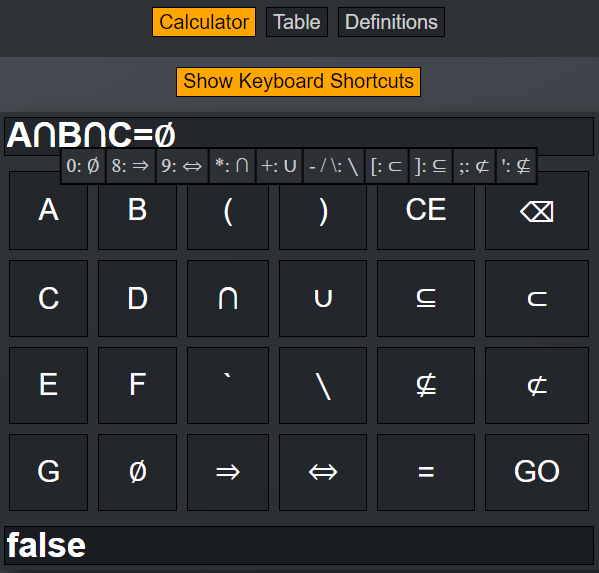
\includegraphics{screenshots/calc.png}
    \caption{Wygląd ekranu kalkulatora}
    \label{fig:calc}
\end{figure}
    
\begin{paragraph}{}
    Ekran kalkulatora to podstawowy ekran aplikacji. Oznacza to, że jest domyślnie widoczny po uruchomieniu aplikacji, oraz że to w nim użytkownik zdanie wejściowe, oraz widzi wynik w postaci prawda albo fałsz. Pozostałe widoki służą zrozumieniu, skąd wziął się wynik, jednak nie są niezbędne do obsługi aplikacji.

    Na samej górze znajdują się trzy przyciski, służące do przełączania między ekranami. Są one elementem wszystkich ekranów. Obecnie wybrany ekran, w tym przypadku ,,Calculator'' jest podświetlony na pomarańczowo. Domyślnie przycisk ,,Table'' jest nieaktywny, ponieważ tabela nie jest wygenerowana zanim użytkownik nie wprowadzi zdania.

    Pasek w którym na zrzucie znajduje się zdanie $A \cap B \cap C = \emptyset$ to wejście aplikacji. Można wprowadzić do niego zdanie przy pomocy znajdujących się poniżej przycisków, lub przycisków na klawiaturze.

    Przycisk ,,Show Keyboard Shortcuts'' służy do wyświetlenia bądź ukrycia okienka znajdującego się między paskiem wejścia aplikacji a przyciskami do jego obsługi. Pokazuje ono pod jakimi klawiszami znajdują się nieoczywiste operacje kalkulatora i domyślnie jest ukryte.

    Pasek na dole z napisem ,,false'' to wyjście aplikacji. Może ono mieć wartość ,,true'', jeżeli wprowadzone zdanie jest tautologią, albo ,,false'', jeżeli nie jest.
\end{paragraph}

\section{Ekran tabeli}
\begin{figure}[h]
    \hspace{1.5cm}
    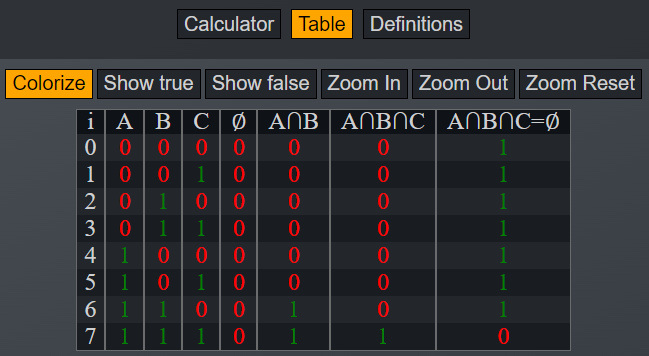
\includegraphics{screenshots/table.png}
    \caption{Ekran z tabelą wygenerowaną dla zdania $A \cap B \cap C = \emptyset$}
    \label{fig:table}
\end{figure}

\begin{paragraph}{}
    Ekran tabeli zawiera przedstawioną graficznię tabelę, utworzoną przez program w celu sprawdzenia, czy podane przez użytkownika zdanie jest tautologią. Może on posłużyć użytkownikowi do zweryfikowania działania programu i zrozumienia jego wyniku. Przypomina się, że sprawdzane zdanie jest tautologią, kiedy ostatnia kolumna tabeli składa się z samych jedynek.

    Liczba wierszy w tabeli rośnie wykładniczo. W związku z tym przeglądanie jej w którymś momencie staje się bardzo niewygodne. W związku z tym nad tabelą umieszczono kilka przycisków, mających na celu ułatwić użytkownikowi korzystanie z tabeli.

    Przycisk ,,Colorize'' koloruje wartości tabeli w sposób przedstawiony na przykładzie, gdzie wartości fałszywe mają kolor czerwony a wartości prawdziwe zielony. Ma to ułatwić przeglądanie tabeli. Domyślnie wartości nie są pokolorowane.

    Przyciski zaczynające się od ,,Show'' służą do pokazywania konkretnych wierszy. Przycisk ,,Show true'' pokazuje tylko wiersze w których ostatnia kolumna ma wartość $1$, a ,,Show false'' tylko wiersze, w których ostatnia kolumna ma wartość $0$.

    Przyciski zaczynające się od ,,Zoom'' służą do zmieniania rozmiaru tabeli. Przycisk ,,Zoom In'' pozwala tabelę przybliżyć, ,,Zoom Out'' oddalić a ,,Zoom Reset'' przywraca jej domyślną wielkość.
\end{paragraph}

\section{Ekran definicji}

\begin{figure}[h]
    \hspace{1.5cm}
    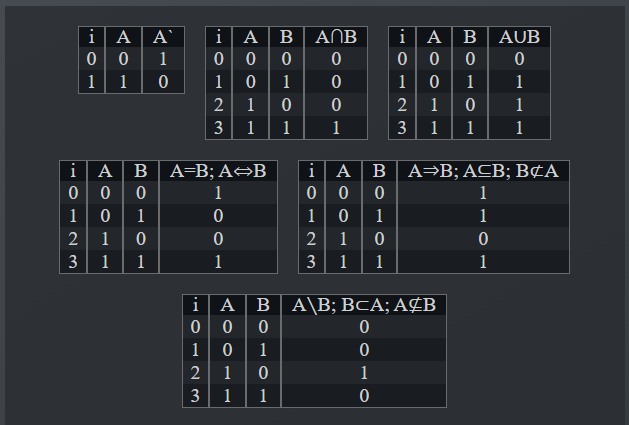
\includegraphics{screenshots/definitions.png}
    \caption{Ekran zawierający tabelki logiczne dla działań na zbiorach}
    \label{fig:definitions}
\end{figure}

\begin{paragraph}{}
    Ekran definicji jest statycznym elementem aplikacji. Oznacza to, że w jego zawartość w~żaden sposób nie ulega zmianie. Zawiera on tabele przedstawiające, w jaki sposób działania na zbiorach mają się do operacji logicznych i ma na celu pomóc użytkownikowi zrozumieć skąd biorą się wartości tabeli w ekranie ,,Table''.
\end{paragraph}

\chapter{Podsumowanie i wnioski}

\begin{paragraph}{}
    Celem pracy było zaprojektowanie oraz implementacja aplikacji webowej służącej do udowadaniania tautologii w teorii zbiorów. Innymi słowy, dla podanego przez użytkownika zdania sprawdzane jest, czy zawsze będzie ono logicznie prawdą. Utworzona na łamach pracy aplikacja miała posiadać przyjazny interfejs w stylu kalkulatora oraz będzie potencjalnie mogła służyć jako pomoc dydaktyczna. Dodatkowym celem pracy było przedstawienie połączenia między logiką a teorią zbiorów oraz okazja do nauki. Opisane w poprzednich rozdziałach podstawy teoretyczne, zaprojektowane na ich podstawie algorytmy, ich realizacja w kodzie oraz ekrany aplikacji pozwalają stwierdzić, że cel ten został zrealizowany.

    Do numerycznego sprawdzania tautologii zaproponowana została w pracy metoda tabelkowa. Oznacza to, że dla wprowadzonego zdania generowana jest tabela wszystkich możliwych wartości logicznych tego zdania, w zależności od wartości logicznych jego składowych. Aplikacja składa się z trzech ekranów. Pierwszy z nich to ekran kalkulatora, służący do wprowadzania zdania oraz wyświetlania wyniku w postaci prawda albo fałsz, informującego, czy zdanie jest tautologią czy nie. Drugi z nich to ekran zawierający wizualizację wygenerowanej przez program tabeli. Trzeci z nich jest statyczny i pokazuje w jaki sposób operacje na zbiorach przekładają się na operacje logiczne.

    Jedną z głównych trudności stworzenia tej aplikacji była możliwość wprowadzenia przez użytkownika dowolnego zdania z dowolnymi działaniami na zbiorach. Sprawdzenie jednego konkretnego zdania przy pomocy kodu jest dużo prostsze.

    Wykorzystana metoda tabelkowa, pomimo prostoty, jest bardzo nieoptymalna pod względem pamięciowym, nawet jeśli, tak jak w tej aplikacji, wartości logiczne przechowywane są na pojedynczych bitach. Wynika to z faktu, że program ma wykładniczą złożoność pamięciową, tzn. jeżeli sprawdzane zdanie ma $n$ zbiorów, wygenerowana tabela ma $2^{n}$ wierszy. Dalej, pomimo, że maksymalna liczba możliwych do wprowadzenia zbiorów równa się liczbie liter na klawiaturze, a zatem liczba wierszy jest ograniczona, to liczba kolumn może być w teorii nieskończona. Wynika to z faktu, że tabela posiada kolumny dla każdej operacji zawartej w podanym zdaniu, nie zostało natomiast wprowadzone żadne ograniczenie co do jego długości. Dodatkowym problemem jest generowanie widoku i wyświetlanie utworzonej przez program tabeli. Dla dużej liczby zbiorów ekran z tabelą generuje się bardzo długo, a~próba jego otwarcia potrafi wyłączyć przeglądarkę. Taka sytuacja nigdy nie miała miejsca dla ekranu kalkulatora, natomiast czas otrzymania wyniku dla bardzo długich zdań sięgał nawet kilkudziesięciu sekund.

    Istnieje kilka potencjalnych sposobów na pozbycie się tego problemu. Ponieważ zdanie nie jest tautologią, jeżeli chociaż w jednym przypadku jest fałszywe, zamiast generować i~sprawdzać całą tabelę od razu, dla dłuższych zdań można ją sprawdzać fragmentarycznie. Podobnie sytuacja ma się w przypadku generowania i wyświetlania jej widoku. Wtedy użytkownik musiałby posiadać możliwość manualnego poinstruowania aplikacji aby wyświetliła dalszą część tabeli.

    Dodatkowo, istnieją łatwiejsze metody implementacji dowodu tabelkowego. Jednym z~nich jest wykorzystanie języka PROLOG. Przy jego pomocy podobny program można stworzyć  o wiele prościej. Przy okazji tej pracy została utworzona wstępna wersja programu w tym języku, ograniczona pod względem dostępnych operacji. Uruchomiona w środowisku SWI-prolog przy okazji sama generowała utworzoną przy obliczeniach tabelę i zwracała poprawny wynik w postaci prawda albo fałsz. Aplikacja ta nie została jednak utworzona w pełni, zatem nie zostało stwierdzone, czy różni się prędkością w porównaniu do stworzonego rozwiązania. Dodatkowo, wykorzystanie języka PROLOG wymagałby utworzenia dodatkowego, przyjaznego użytkownikowi interfejsu, ponieważ w swojej podstawowej wersji jest on ciężki w obsłudze.

    Opisany wyżej program wykorzystujący PROLOG wciąż jednak wykorzystuje metodę tabelkową. Autorowi nie są znane inne metody numerycznego dowodzenia tautologii w rachunku zbiorów. Na przyszłośc więc, podstawowym ulepszeniem stworzonej aplikacji byłoby poszukanie innych, bardziej optymalnych sposobów dowodzenia tautologii oraz ich implementacja, z zachowaniem obecnego interfejsu. W przypadku nieznalezienia alternatyw, lub niemożności ich implementacji, można spróbować stworzyć aplikację od zera wykorzystując PROLOG i porównać czasy działania. Dla aplikacji w obecnej formie, ponieważ ma ona stanowić potencjalną pomoc dydaktyczną, warto by utworzyć dodatkowe widoki, które lepiej tłumaczą jej działanie, np. przedstawić realizowany przez aplikację proces konwersji podanego przez użytkownika zdania do Odwrotnej Notacji Polskiej.

    Aplikacja opisana w tym dokumencie, wraz z dokumentem oraz kodem i źródłami \LaTeX \\wykorzystanymi do ich utworzenia znajdą się w całości na moim koncie GitHub~\cite{github:aglebionek}.
\end{paragraph}


\nocite{*} % Wyświetl bibligrafię bez względu na to czy jest cytowana czy nie

\bibliographystyle{unsrt}
\bibliography{bibliography}
%\addcontentsline{toc}{chapter}{\bibname}

\beforelastpage

\end{document}
